\documentclass{article}
\usepackage[UTF8]{ctex}
\usepackage{amsmath,amsthm,amssymb,amsfonts}
\usepackage{bm}
\usepackage{geometry}
\usepackage{booktabs}
\usepackage{graphicx}
\usepackage{caption}
\usepackage{hyperref}
\usepackage{color}
\hypersetup{hidelinks,
	colorlinks=true,
	allcolors=blue,
	pdfstartview=Fit,
	breaklinks=true}
\usepackage{algorithm}
\usepackage{listings}
\usepackage{minted}

\lstset{
    numbers=left, %在左侧显示行数
  breaklines,%自动换行
  columns=flexible,%不随便添加空格,只在已经有空格的地方添加空格,
%如果想要添加空格使用fixed作为参数(这是默认的),如果坚决不添加空格使用fullflexible作为参数.
}

\setlength{\parindent}{0pt}
\geometry{a4paper,left=2.5cm,right=2.5cm,top=2cm,bottom=2cm}

\title{\textbf{\huge{Monte Carlo Method预测中国股价}}}
\date{\today}
\author{王炽 21307110146 \\ 杨珩 21300680048}

\begin{document}
    \maketitle
    \section{内容介绍}
    \qquad 本作业通过对上证50指数的成分股的历史数据分析,估计了其成分股的价格波动参数,
    在每只成分股的股价均为几何布朗运动的假设下,合理考虑个股之间的波动率关系,
    最终采用蒙特卡洛法预测个股变动,以此预测上证50指数变化。
    \section{数据来源}
    \subsection{股票价格}
    \qquad 本报告中股票价格的历史数据自2021年1月1日起至2024年4月11日,在本报告涉及的股票样本中,仅有三峡能源(上市于2021年6月10日),
    海光信息(上市于2022年8月12日)和中国电信(2021年8月20日在上交所上市)三只股票缺乏早期部分数据。所有选中的股票的数据均超过300个交易日。

    \qquad  股票价格选择的是每个交易日的收盘价,为保证价格连续性,已经提前进行了后复权处理,数据直接来源是wind咨询。
    \subsection{成分股和权重}
    \qquad 根据上证50指数编制的相关规定,定期调样频率为每半年一次,上次调样时间为2023年12月11日,下次定期调样在2024年六月,超出本报告
    预测的时间范围,因此本报告直接选择当前的成分股进行估计。
    
    \qquad 考虑各成分股权重采用的是调整市值\footnote{参考\href{https://www.csindex.com.cn/indices/family}{中证指数有限公司官网(https://www.csindex.com.cn/indices/family)}的编制说明},计算方法复杂,
    而短期之内市值变化不大,因此直接选用中证指数有限公司最近一次披露交易日(2024年3月29日)作为权重。
    \section{模型介绍}
    \subsection{单只股票的几何布朗运动}
    \qquad 假设对于某只股票的股价$S_t$,遵循一个几何布朗运动:
    \begin{align}
        dS_t=\mu S_tdt+\sigma S_tdW_t
    \end{align}
    \qquad $W_t$表示布朗运动,即$dW_t\sim N(0,dt)$,假设股价的对数为$f(S,t)=lnS$,考虑对股价的对数做泰勒展开:
    \begin{align}
        df(S,t)=\frac{\partial f}{\partial S}dS+\frac{\partial f}{\partial t}dt+\frac{\partial^2 f}{2\partial S^2}dS^2+O(df)
    \end{align}
    \qquad 由于$\frac{\partial f}{\partial S} = \frac{1}{S}$,$\frac{\partial f}{\partial t}=0$,$\frac{\partial^2 f}{\partial S^2}=-\frac{1}{S^2}$,此时(2)式可改写为:
    \begin{align}
        df(S,t)&=\frac{dS}{S}-\frac{dS^2}{2S^2}\nonumber\\
        &=\mu dt+\sigma dW-\frac{1}{2}\sigma^2dW^2+O(df)
    \end{align}
    \qquad 考虑到在积分时,布朗运动$dW^2=dt$,因此,对(3)式两边积分:
    \begin{gather}
        \int_{t}^{T}\,dlnS=\int_{t}^{T}(\mu-\frac{\sigma^2}{2})\,dt+\int_{t}^{T}\sigma dW\\
        lnS_T-lnS_t=(\mu-\frac{\sigma^2}{2})(T-t)+\sigma\epsilon\sqrt{T-t} 
    \end{gather}
    \qquad 上式中,$\epsilon$是一个标准正态分布随机变量,也是蒙特卡洛模拟的主要内容。
    \subsection{多只股票的联合布朗运动}
    \qquad 假如对于多只股票,他们的\textcolor{red}{\textbf{收益率}}遵循多元正态分布:
    \begin{align}
        \boldsymbol{X} = (X_1,X_2,\cdots,X_n)\sim N(\boldsymbol{\mu},\varSigma)
    \end{align}
    \qquad 通过Cholesky分解,转换为标准形式:
    \begin{gather}
        \boldsymbol{X} = \boldsymbol{\mu}+AZ,\ where\ AA^T=\varSigma,\ Z\sim N(0,I) \\
        A=\begin{pmatrix}
            a_{11}&0&\cdots&0\\
            a_{21}&a_{22}&\cdots&0\\
            \vdots&\vdots&\ddots&\vdots\\
            a_{n1}&a_{n2}&\cdots&a_{nn}
        \end{pmatrix}\nonumber
    \end{gather}
    \qquad 带入上一部分的布朗运动,我们假设对于多支股票的股价:
    \begin{align}
        \boldsymbol{X}=\begin{pmatrix}
            \frac{dS_1}{S_1}\\
            \frac{dS_2}{S_2}\\
            \vdots\\
            \frac{dS_n}{S_n}
        \end{pmatrix}=\begin{pmatrix}
            \mu_1\\
            \mu_2\\
            \vdots\\
            \mu_n
        \end{pmatrix}dt+A\begin{pmatrix}
            dW_1\\
            dW_2\\
            \vdots\\
            dW_n
        \end{pmatrix}
    \end{align}
    \qquad 对于其中任何一只股票的价格,同样采用上面的方法表达:
    \begin{gather}
        dS_{i,t}=\mu_i S_{i,t}dt+S_{i,t}\sum_{j=1}^{i}a_{ij}dW_{j,t}
    \end{gather}
    \qquad 和上一部分一样,对股价的对数进行泰勒展开:
    \begin{align}
        df(S_i,t)&=\frac{dS_i}{S_i}-\frac{dS_i^2}{2S_i^2}\nonumber\\
        &=\mu_i dt+\sum_{j=1}^{i}a_{ij}dW_{j}-\frac{1}{2}\left(\sum_{j=1}^{i}a_{ij}dW_{j}\right)^2+O(df)
    \end{align}
    \qquad 此时的多个布朗运动之间,$dW_i^2=dt$,而考虑前文公式(7)中对收益率的分解$\boldsymbol{X} = \boldsymbol{\mu}+AZ$,由于$\boldsymbol{Z}$是多个
    独立的正态分布,因此,在考虑股价几何布朗运动时,(8)式中的$W_1,W_2,\cdots,W_n$全部独立,而两个独立的布朗运动的协变差为0,即$dW_jdW_j=0$,此时对(10)式两边积分:
    \begin{gather}
        \int_{t}^{T}\,dlnS_i=\int_{t}^{T}(\mu_i-\dfrac{\sum_{j=1}^{i}a_{i,j}^2}{2})\,dt+\sum_{j=1}^{i}\int_{t}^{T}a_{i,j} dW_j\\
        lnS_{i,T}-lnS_{i,t}=(\mu_i-\dfrac{\sum_{j=1}^{i}a_{i,j}^2}{2})(T-t)+\sum_{j=1}^{i}a_{i,j}\sqrt{T-t}\epsilon_j 
    \end{gather}
    \qquad 上式中,$\epsilon_1,\epsilon_2,\cdots,\epsilon_n$是$n$个独立的标准正态分布随机变量,也是蒙特卡洛模拟的主要内容。将上述式子重新改写成向量形式:
    \begin{align}
        \overrightarrow{lnS_{i,T}-lnS_{i,t}}&=(T-t)\boldsymbol{\mu}-\frac{1}{2}(T-t)A\circ A\boldsymbol{I_{n\times 1}}+\sqrt{T-t}\boldsymbol{\epsilon}A^T\\
        \text{where,}\qquad\qquad\qquad\nonumber\\
        \qquad\boldsymbol{\mu}&= (\mu_1,\mu_2,\cdots,\mu_n)^T\nonumber\\
        \qquad\boldsymbol{I_{n\times1}}&= (1,1,\cdots,1)^T\nonumber\\
        \qquad\boldsymbol{\epsilon}&= (\epsilon_1,\epsilon_2,\cdots,\epsilon_n)^T\nonumber
    \end{align}
    \section{程序实现}
    \qquad 本部分内容基于python实现,预测去间为自4月12日开始的10个交易日上证50指数。项目仓库地址:\href{URL}{text}。
    \subsection{历史数据处理}
    \qquad 原始数据表(xlsx和csv)已预先经过处理,转换为便于读取的feather轻量数据,具体处理方法和源文件均已上传至github仓库。
    \begin{listing}[htb]
        \caption{历史数据处理}
        \begin{minted}[breaklines,linenos,numbersep=-1em,baselinestretch=1.1]{python3}
    import pandas as pd
    import numpy as np
    #读取收盘价,个股权重,指数数据
    close = pd.read_feather('close.txt').set_index('date')
    weight = pd.read_feather('weight.txt')
    index = pd.read_feather('000016.txt').set_index('date')
    #计算每个交易日的收益率(收盘价已复权,可以直接计算)
    ret = (close - close.shift(1)) / close
    #历史平均收益率
    mu_vec = ret.mean()
    #历史收益率的协方差矩阵
    varSigma = ret.cov()
    #cholesky分解
    A_cholesky = np.linalg.cholesky(np.array(varSigma))
    \end{minted}
    \end{listing}
    \subsection{蒙特卡洛模拟}
    \begin{listing}[htb]
        \caption{蒙特卡洛模拟}
        \begin{minted}[breaklines,linenos,numbersep=-1em,firstnumber=31,baselinestretch=1]{python3}
    def monte_carlo_simulate():
        # 生成50组标准正态随机变量,每组10个
        epsilon_m = []
        for i in range(50):
            epsilon_m.append(np.random.normal(loc=0.0, scale=1.0, size=10))
        epsilon_m = np.array(epsilon_m)

        # 分10天,每天50个随机变量,用于模拟个股收益率
        ret_sim = []
        for epsilon_vec in epsilon_m.T:
            #计算联合布朗运动方程向量形式,即前一部分公式(13)的右半部分
            ret_log_vec = mu_vec-0.5*A_cholesky*A_cholesky@(np.ones(50).T) + A_cholesky@epsilon_vec
            ret_sim.append(np.exp(ret_log_vec))
        ret_sim = pd.DataFrame(ret_sim)
        # 返回五十支股票的(收益率+1)矩阵
        return ret_sim
    \end{minted}
    \end{listing}
    \subsection{模拟上证50指数结果}
    \begin{listing}[htb]
        \caption{拟合指数绘图}
        \begin{minted}[breaklines,linenos,numbersep=-1em,firstnumber=15,baselinestretch=0.9]{python3}
    #导入绘图库并设置
    import matplotlib.pyplot as plt
    plt.rcParams['font.sans-serif'] = ['SimHei']
    plt.figure(figsize=(12,6),dpi=400)
    plt.xlabel('日期',fontsize=15)
    plt.ylabel('000016.SH',fontsize=15)
    #画历史数据
    index_history = index.head(15)['close'].iloc[::-1]
    index_history.index = [k[5:] for k in index_history.index]  
    plt.plot(index_history,marker='.',label='历史数据',color='black',linewidth=2)
    #画预测数据(这里30表示30组)
    for i in range(1):
        ret_sim = monte_carlo_simulate()
        weight.index = weight['code'].astype(str)
        index_ret_sim = weight['weight']* ret_sim * 0.01
        index_sim = index_ret_sim.T.sum() * index['close'][0]
        index_sim.index = ['4/12','4/15','4/16','4/17','4/18','4/19','4/22','4/23','4/24','4/25']
        index_sim['4/11']=index['close'][0]
        index_sim = index_sim.sort_index()
        plt.plot(index_sim)
    plt.vlines('4/11',2300,2450,colors='red',linestyles='dashed')
    \end{minted}
    \end{listing}
    \qquad 单次拟合结果如图\ref{sim1}所示,而多次拟合(30次)结果如图\ref{sim2}所示,特别的,红色虚线左边表示历史数据,右边则是模拟数据。
    \begin{figure}[htbp]
        \centering
        \caption{单次模拟000016结果}
        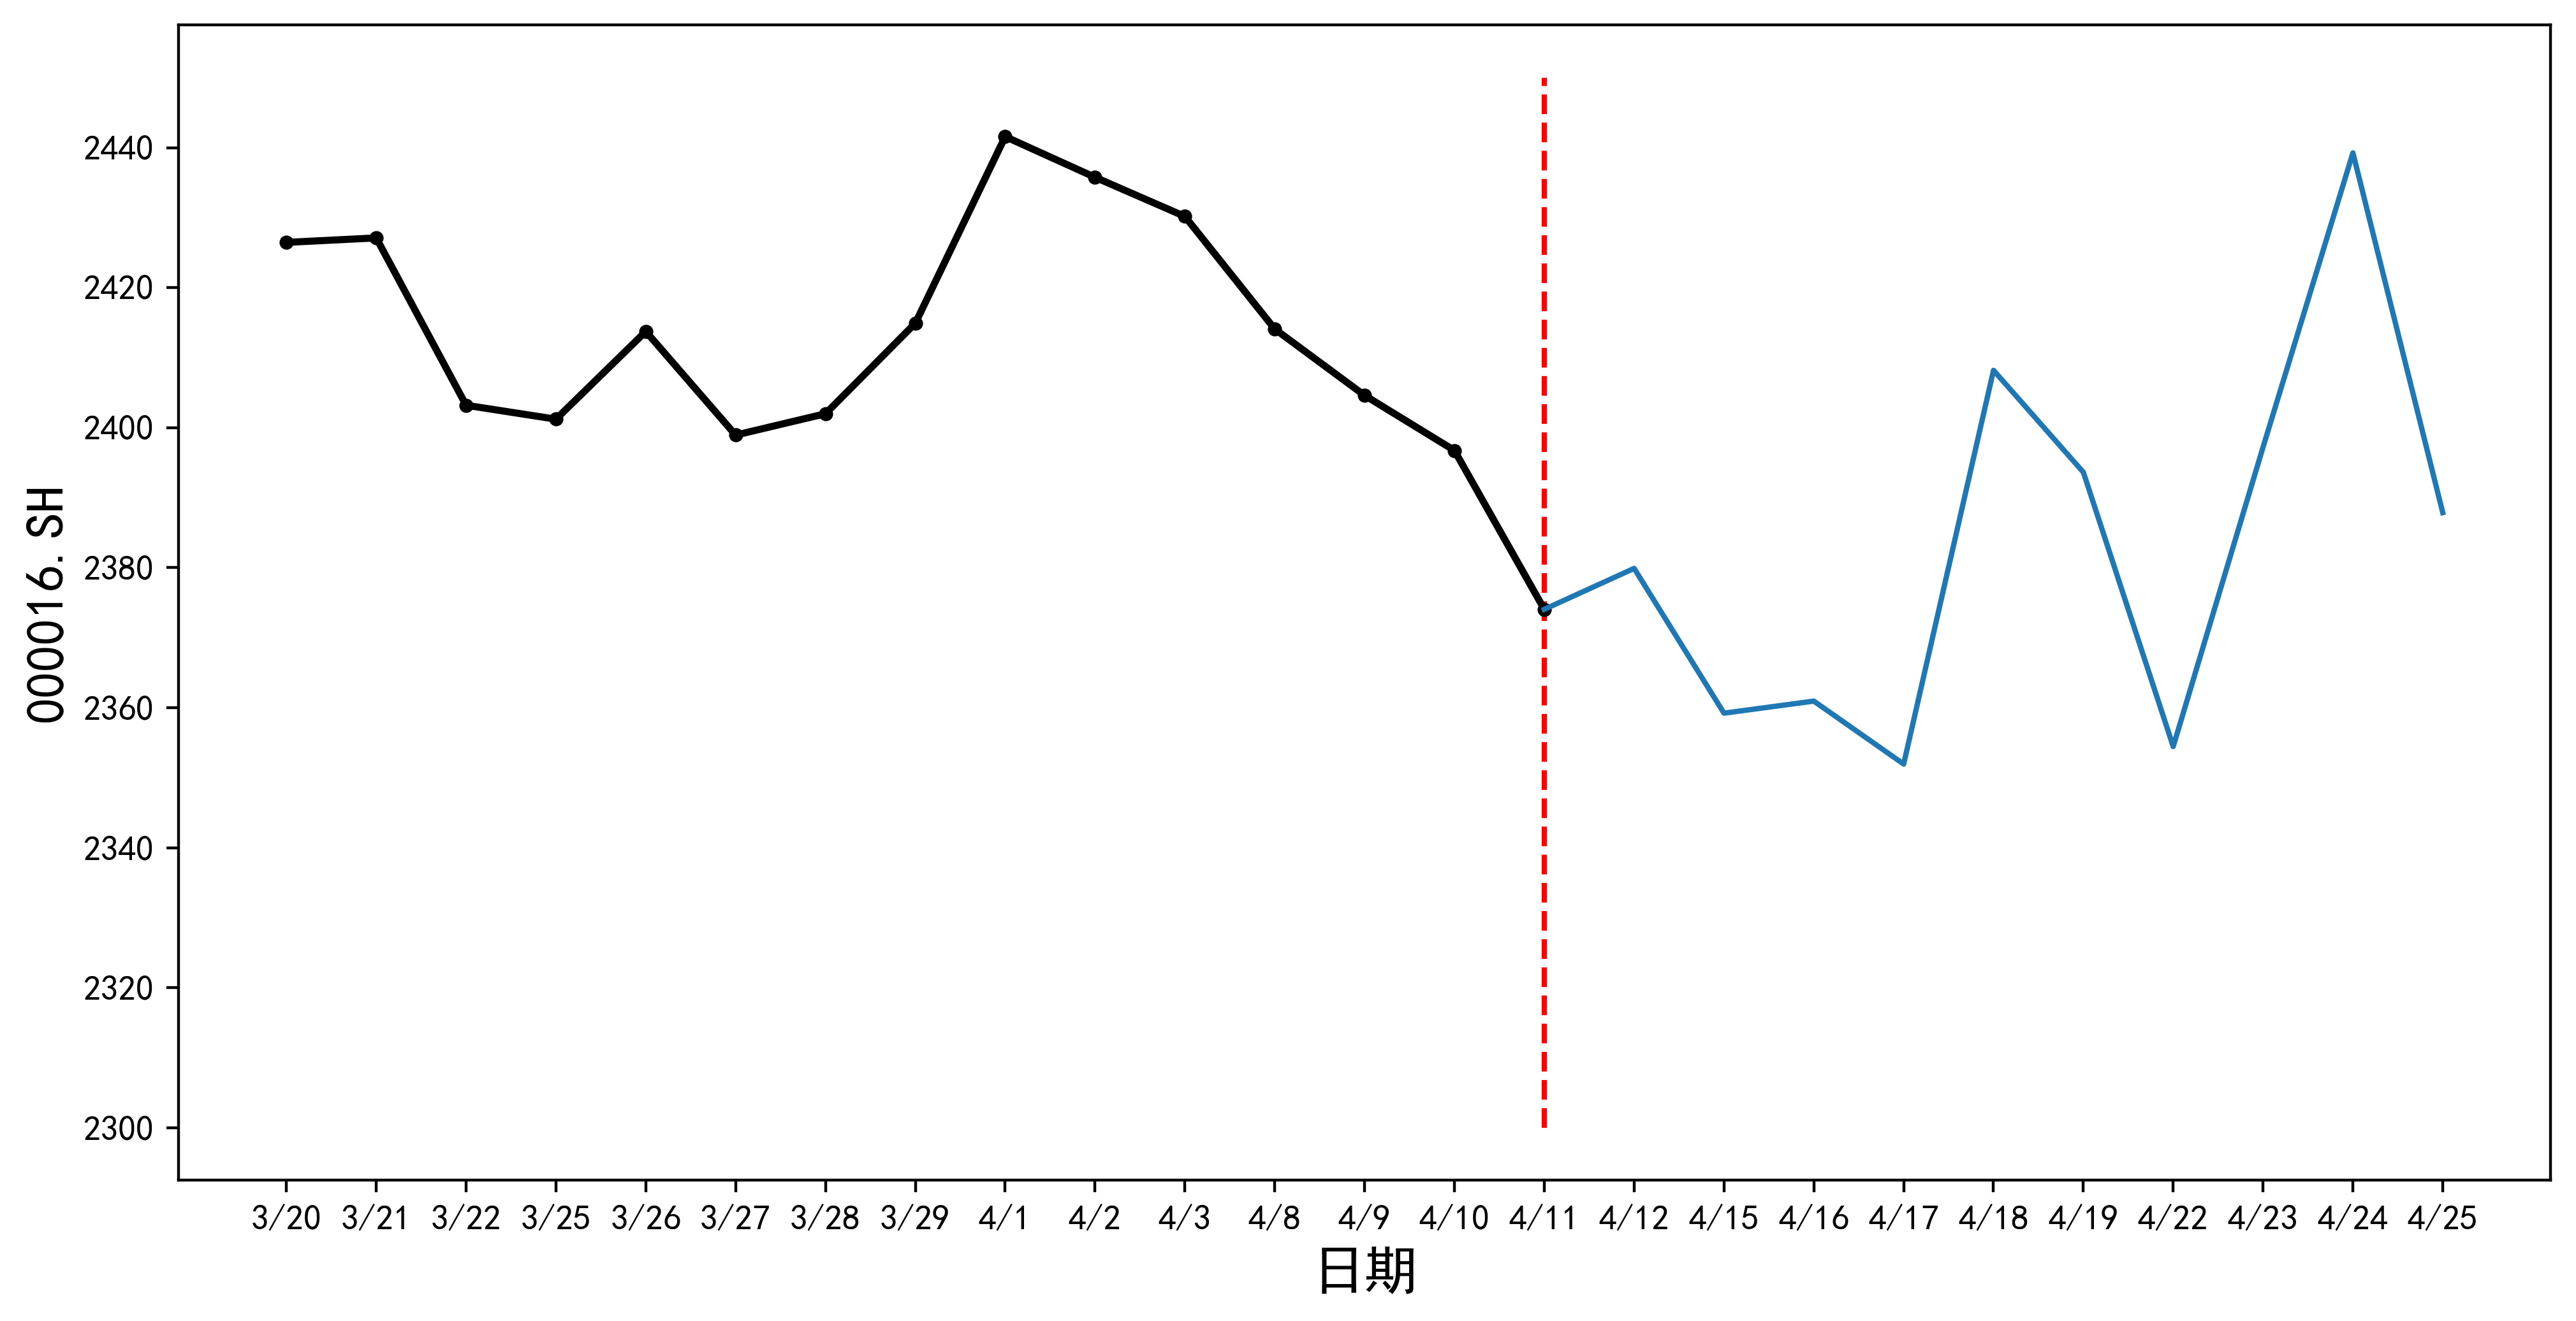
\includegraphics[width=\textwidth]{figure/sim1.png}
        \label{sim1}
    \end{figure}
    \begin{figure}[htbp]
        \centering
        \caption{三十次模拟000016结果}
        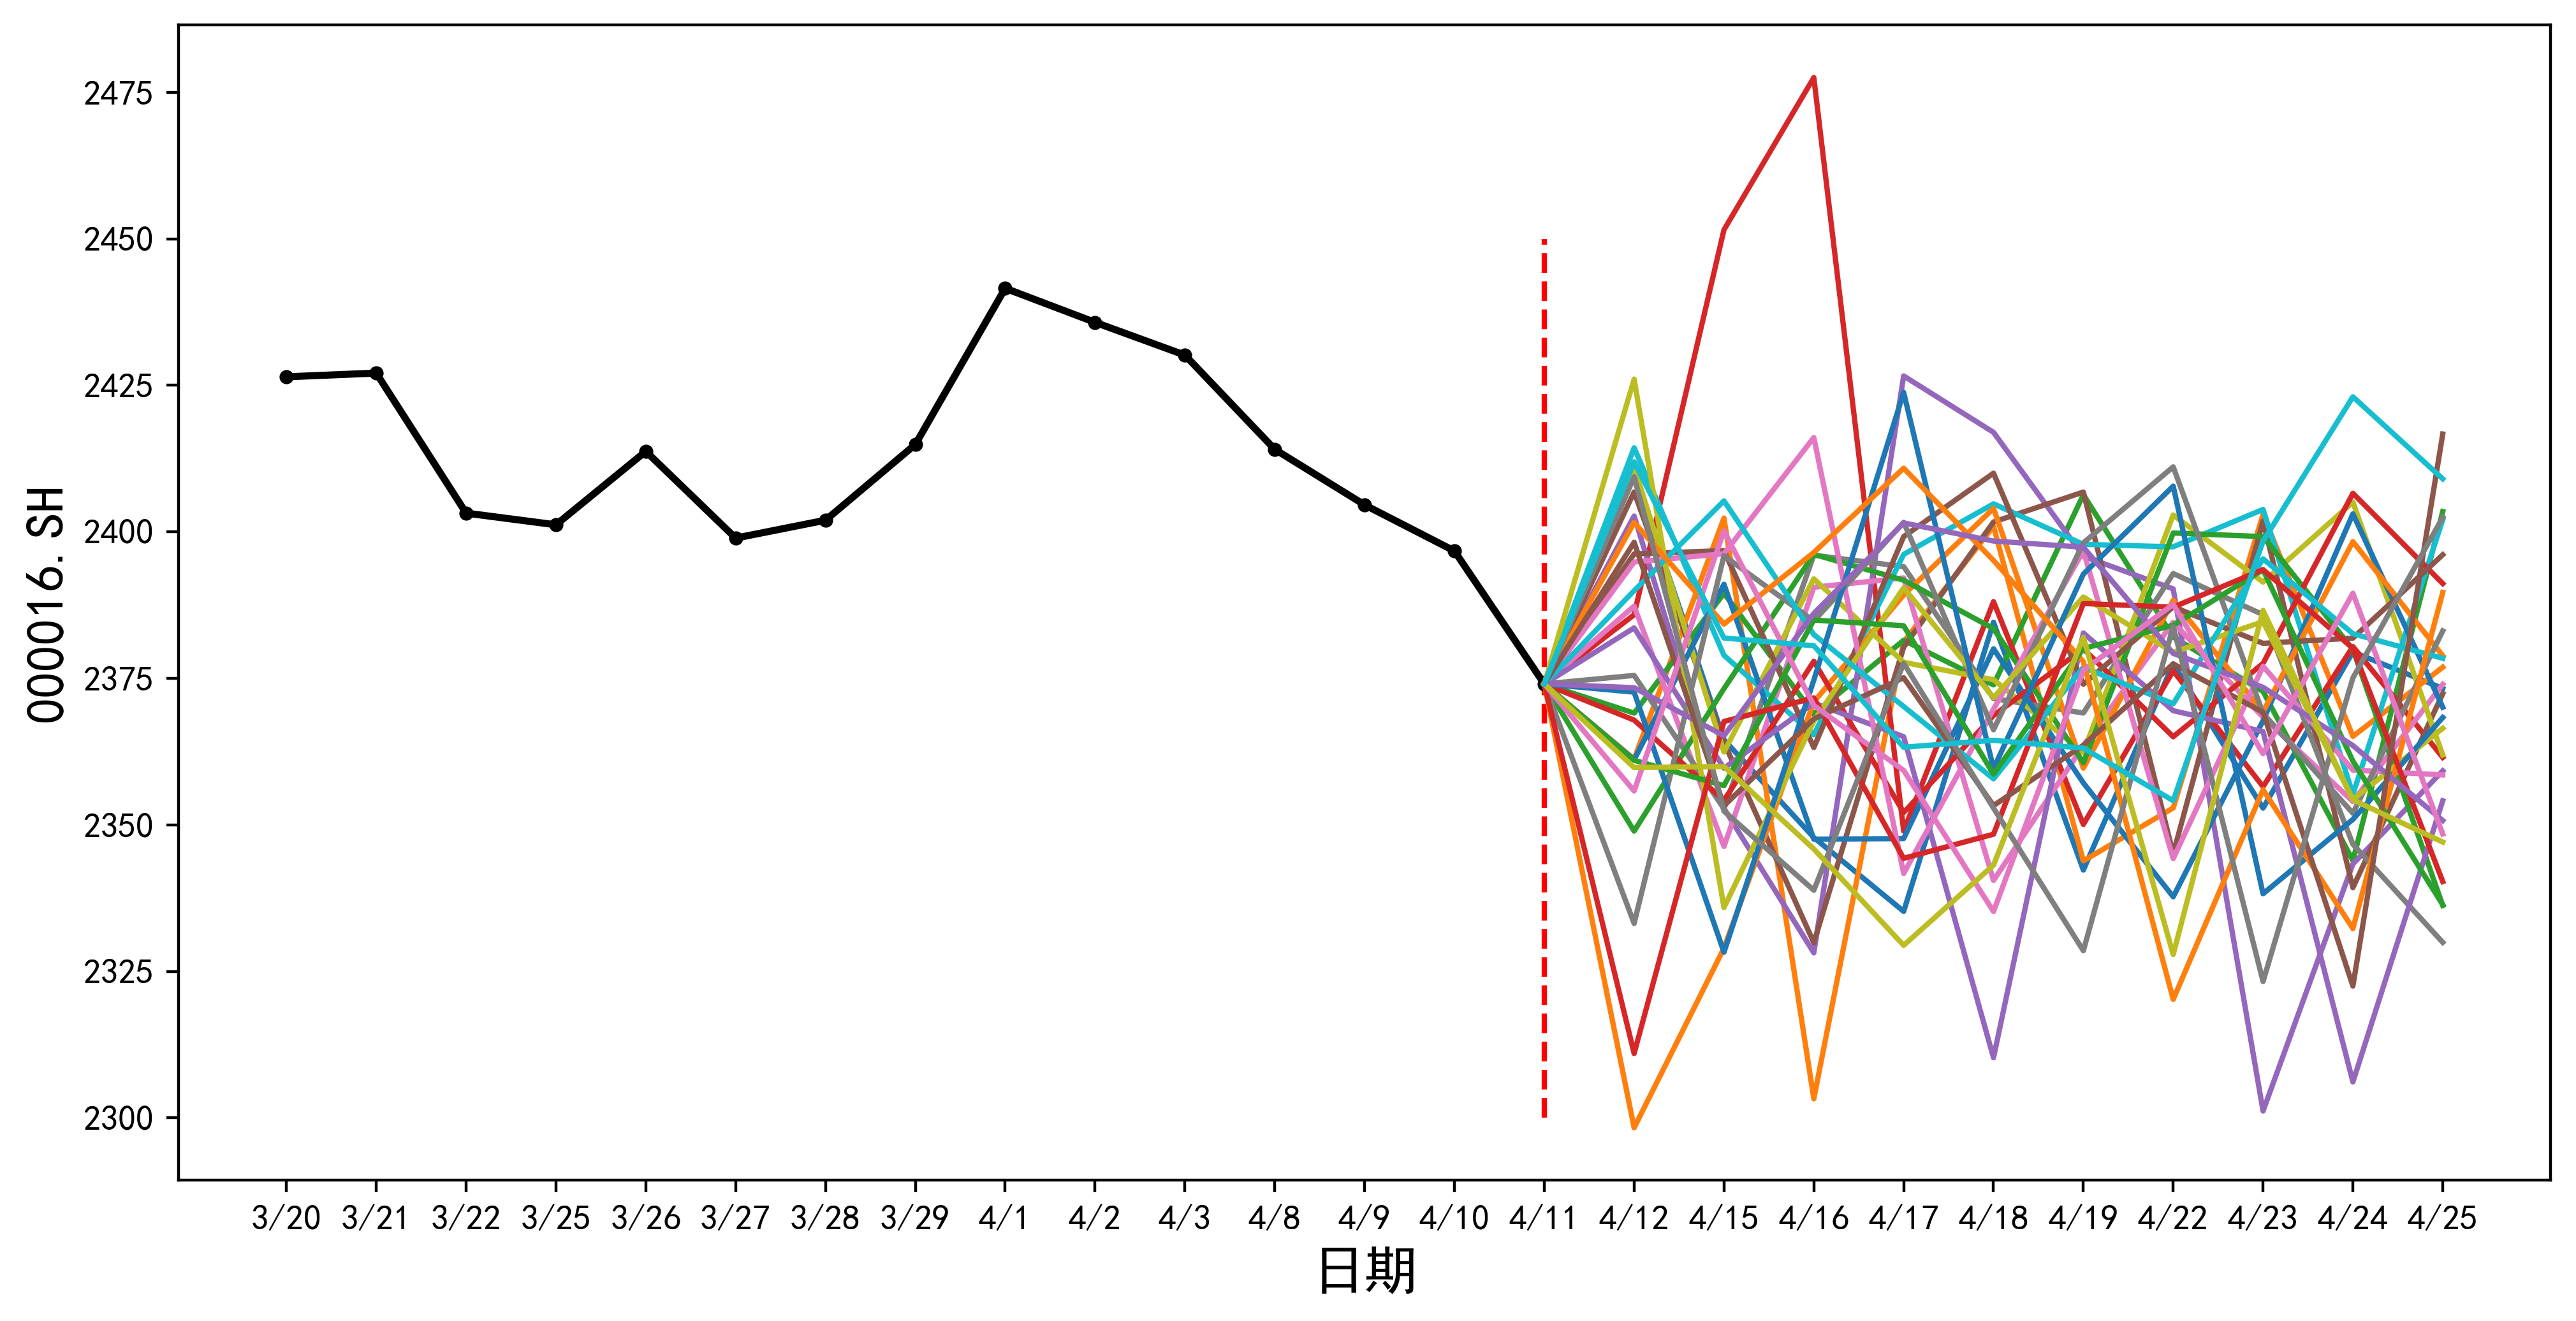
\includegraphics[width=\textwidth]{figure/sim2.png}
        \label{sim2}
    \end{figure}


\end{document}